\documentclass[border={0.1cm 0.1cm 0.1cm 0.1cm}]{standalone}  %E,S,W,N

\usepackage{amssymb}
\usepackage{amsmath}
\usepackage{tikz}
\usetikzlibrary{shapes} %for node shapes
\usetikzlibrary{calc}	%for centerarc
\usetikzlibrary{decorations.text,decorations.markings} %for bendy text

\def\centerarc[#1](#2)(#3:#4:#5) {\draw[#1] ($(#2)+({#5*cos(#3)},{#5*sin(#3)})$) arc (#3:#4:#5);}

\begin{document}
	
	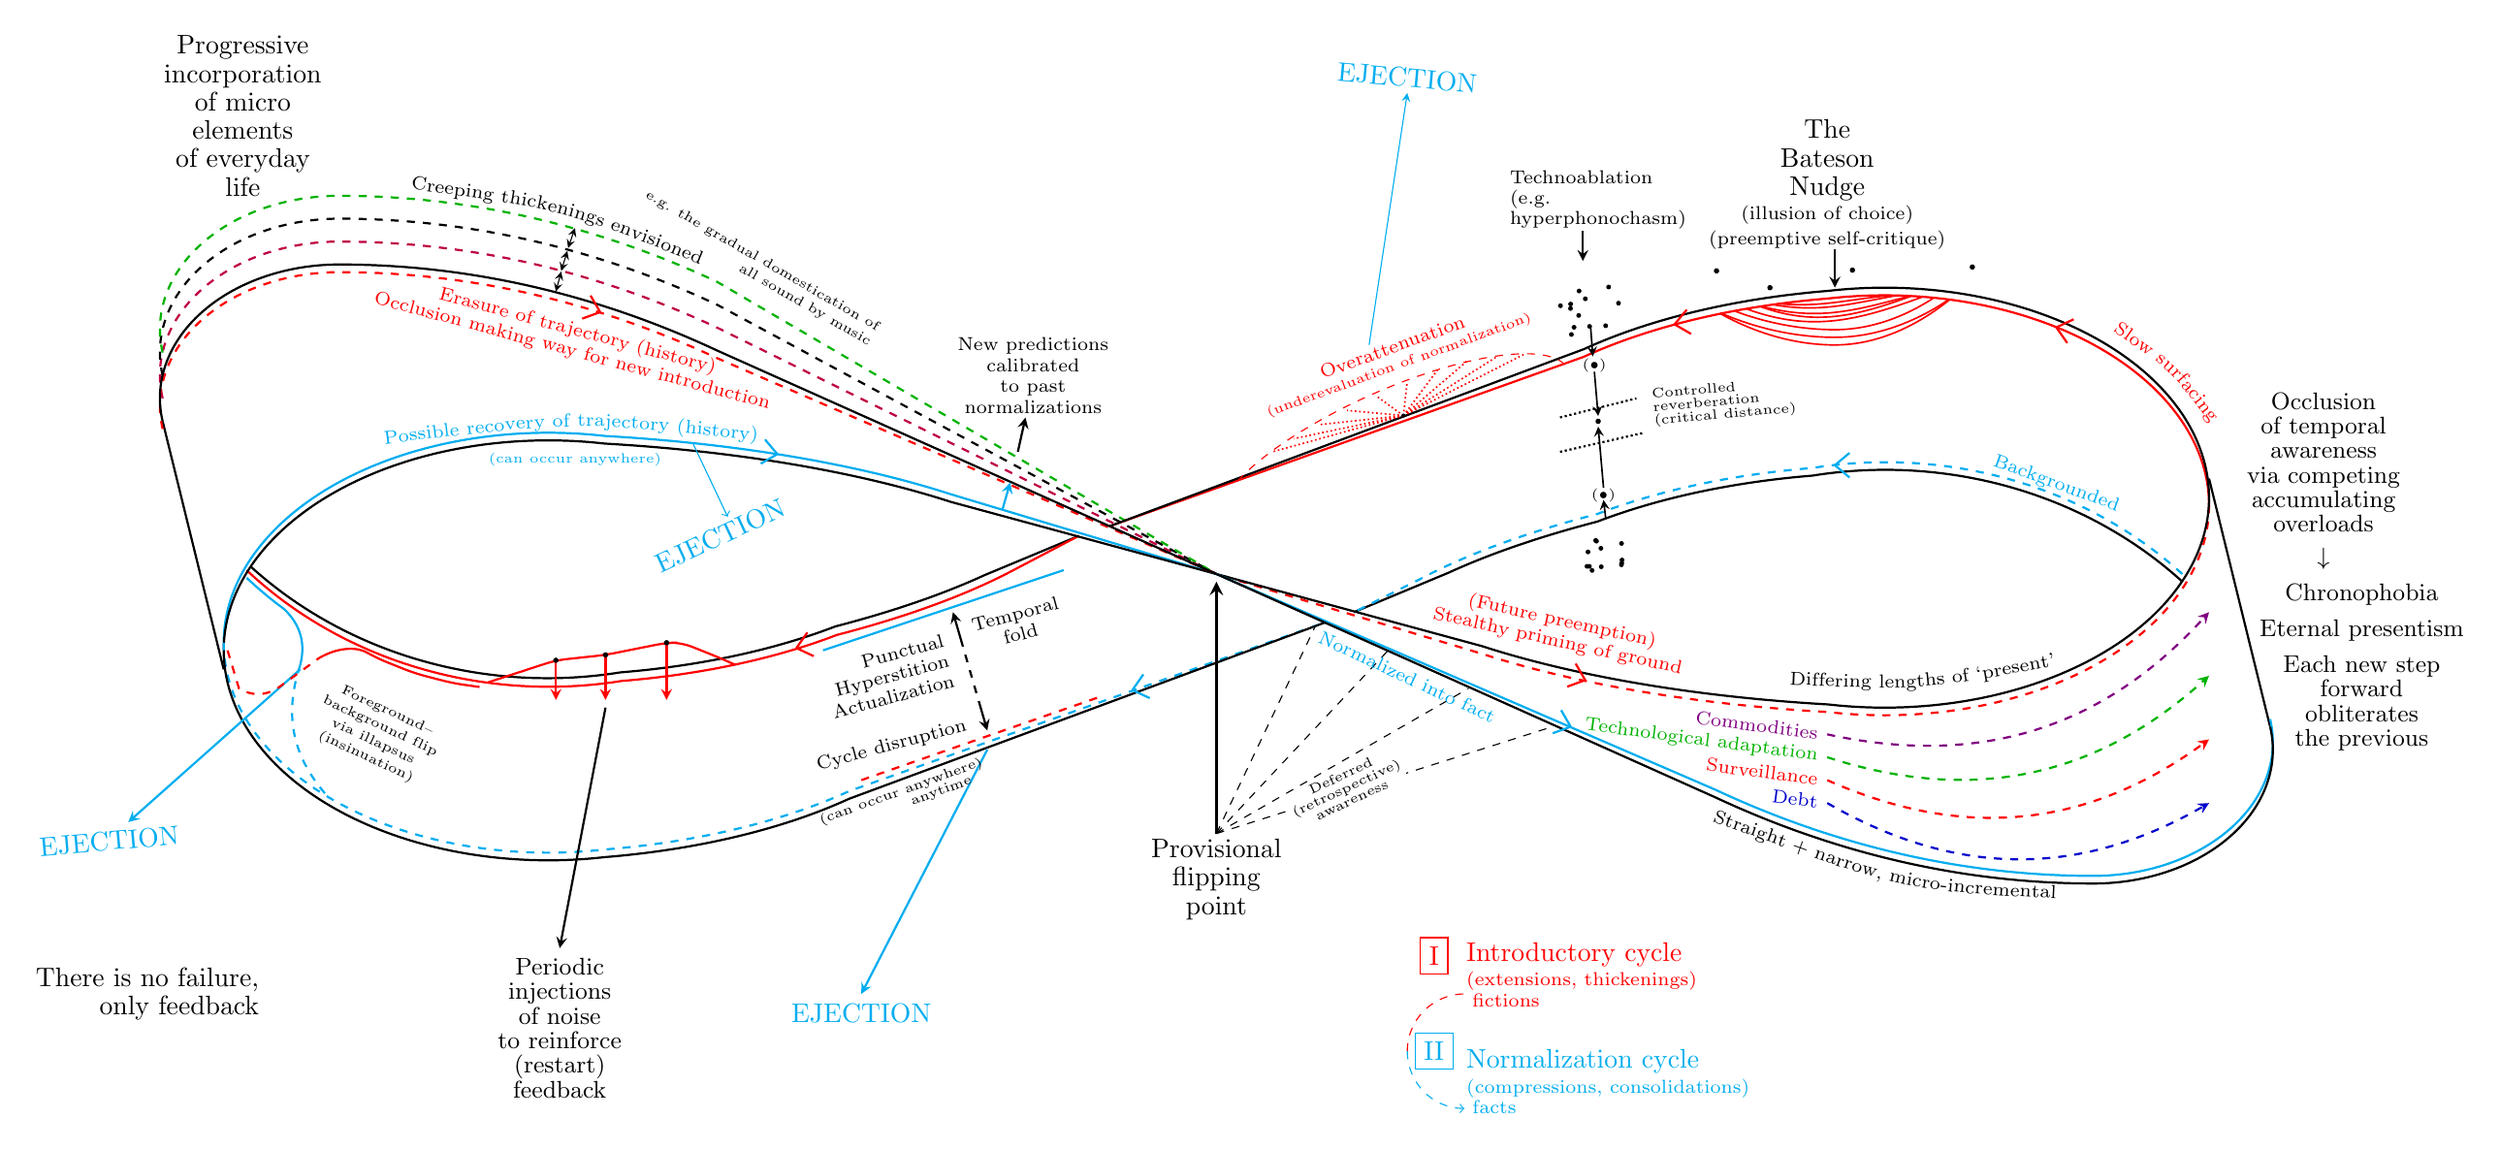
\begin{tikzpicture}	
	%LEFT SIDE
	\draw[thick] (-12.65,0.1) arc (225:280:5.5 and 5) arc (280:310:6 and 2.75) arc (310:326:10.5 and 3.25) -- (-1.8,0.5);
	\draw[thick,red] (-12.65-0.05,0.05) arc (224:280:5.5 and 5) arc (280:310:6 and 2.75) arc (310:330:10.5 and 3.25) -- (-1.8,0.5);
	%
	\draw[thick,cyan] (-13,-0.9) arc (180:80:4.25 and 2.75) arc (80:45:8.5 and 2.75) -- (0,0);
	\draw[thick] (-13,-1) arc (180:80:4.25 and 2.75) arc (80:45:8.5 and 2.75) -- (0,0);
	%
	\draw[thick,cyan,dashed] (-13,-0.9) arc (180:280:4.25 and 2.75) arc (280:315:6 and 2.75) -- (1.45,-0.625);
	\draw[thick] (-13,-1) arc (180:280:4.25 and 2.75) arc (280:315:6 and 2.75) -- (1.45,-0.625);
	%
	\draw[thick,purple,dashed] (-13.8,2.3) arc (190:90:2.35 and 1.75) arc (90:72:16 and 23) -- (0,0);
	\draw[thick,dashed] (-13.8,2.6) arc (190:90:2.35 and 1.75) arc (90:72:16 and 23) -- (0,0);
	\draw[thick,green!70!black,dashed] (-13.8,2.9) arc (190:90:2.35 and 1.75) arc (90:72:16 and 23) -- (0,0);
	%
	\draw[thick] (-13,-1.25)--(-13.8,2);
	\draw[thick,red,dashed] (-13.8,1.9) arc (190:90:2.35 and 1.75) arc (90:72:16 and 23) -- (0,0);
	\draw[thick] (-13.8,2) arc (190:90:2.35 and 1.75) arc (90:72:16 and 23) -- (0,0);
	
	%RIGHT SIDE
	\draw[thick,xscale=-1,yscale=-1] (-12.65,0.1) arc (225:280:5.5 and 5) arc (280:310:6 and 2.75) arc (310:326:10.5 and 3.25) -- (-1.8,0.5);
	\draw[thick,cyan,dashed,xscale=-1,yscale=-1] (-12.65,0) arc (225:280:5.5 and 5) arc (280:310:6 and 2.75) arc (310:330:10.5 and 3.25) -- (-1.8,0.5);
	%
	\draw[thick,red,xscale=-1,yscale=-1] (-13,-0.9) arc (180:280:4.25 and 2.75) arc (280:315:6 and 2.75) -- (1.4,-0.625);
	\draw[thick,xscale=-1,yscale=-1] (-13,-1) arc (180:280:4.25 and 2.75) arc (280:315:6 and 2.75) -- (1.4,-0.625);
	%
	\draw[thick,red,dashed,xscale=-1,yscale=-1] (-13,-0.9) arc (180:80:4.25 and 2.75) arc (80:45:8.5 and 2.75) -- (0,0);
	\draw[thick,xscale=-1,yscale=-1] (-13,-1) arc (180:80:4.25 and 2.75) arc (80:45:8.5 and 2.75) -- (0,0);
	%
	\draw[thick,xscale=-1,yscale=-1] (-13,-1.25)--(-13.8,2);
	\draw[thick,cyan,xscale=-1,yscale=-1] (-13.8,1.9) arc (190:90:2.35 and 1.75) arc (90:72:16 and 23) -- (0,0);
	\draw[thick,xscale=-1,yscale=-1] (-13.8,2) arc (190:90:2.35 and 1.75) arc (90:72:16 and 23) -- (0,0);
	
	%LABELS
	\node[align=right] at (-14,-5.5) {There is no failure,\\[-0.5mm] only feedback};
	
	\draw[thick,cyan,->,>=stealth] (-12,-1.25)--(-14.25,-3.25);
	\node[align=center,cyan,rotate=5] at (-14.5,-3.5) {EJECTION};
	
	\node[align=center,rotate=-25] at (-11,-2.1) {\tiny Foreground--\\[-2mm]\tiny background flip \\[-2mm]\tiny via illapsus \\[-2mm]\tiny (insinuation)};
	
	\node[align=center] at (-12.75,6) {Progressive\\[-0.5mm] incorporation \\[-0.5mm] of micro \\[-0.5mm] elements \\[-0.5mm] of everyday \\[-0.5mm] life};
	
	\draw[thick,->,>=stealth] (-8,-1.75)--(-8.6,-4.9) node[align=center,below] {\small Periodic\\[-1mm] \small injections\\[-1mm] \small of noise\\[-1mm] \small to reinforce\\[-1mm] \small (restart)\\[-1mm] \small feedback};
	
	%INJECTIONS OF NOISE
	\draw[thick,red,rounded corners] (-9.54,-1.42)--(-8.65,-1.13)--(-8,-1.06)--(-7.2,-0.9)--++(0.2,0)--(-6.5,-1.1)--(-6.3,-1.19);
	\draw[thick,->,>=stealth,red] (-8.65,-1.13)--(-8.65,-1.65);	\fill (-8.65,-1.13) circle (1pt);
	\draw[thick,->,>=stealth,red] (-8,-1.06)--(-8,-1.65); 		\fill (-8,-1.06) circle (1pt);
	\draw[thick,->,>=stealth,red] (-7.2,-0.9)--(-7.2,-1.65);		\fill (-7.2,-0.9) circle (1pt);
	
	%WARPED LINES
	\draw[thick,cyan] (-12.65-0.05,-0.05) arc (224:231:5.5 and 5) to[bend left] (-12,-1.2);
	\draw[thick,cyan,dashed] (-12,-1.2) to[bend right] (-11.65,-2.9);
	\draw[thick,red,dashed] (-12.95,-1)--(-12.8,-1.5) to[bend right] (-12.3,-1.5)--(-11.75,-1.1);
	\draw[thick,red,rounded corners] (-11.75,-1.1) to[bend left] (-11,-1.1)--(-10.5,-1.3)--(-10,-1.43)--(-9.65,-1.48);
	%----------------------------
	%LEFT
	
	\node[align=center] at (0,-4) {Provisional \\[-0.5mm] flipping \\[-0.5mm] point};
	\draw[very thick,->,>=stealth] (0,-3.4)--(0,-0.1);
	\draw[dashed] (0,-3.4)--(1.3,-0.675);
	\draw[dashed] (0,-3.4)--(2.25,-1);
	\draw[dashed] (0,-3.4)--(3.3,-1.5);
	\draw[dashed] (0,-3.4)--(4.4,-2);
	
	\node[cyan,rotate=-25] at (2.5,-1.35) {\scriptsize Normalized into fact};
	\node[align=center,rotate=25,fill=white,inner sep=0.5] at (1.7,-2.8) {\tiny Deferred \\[-2.5mm] \tiny (retrospective) \\[-2.5mm]\tiny awareness};
	
	\draw[<->,>=stealth] (-8.65,3.7)--(-8.58,3.96);
	\draw[<->,>=stealth] (-8.58,3.97)--(-8.5,4.23);
	\draw[<->,>=stealth] (-8.49,4.27)--(-8.4,4.53);
	\node[align=center,red,rotate=-15] at (-8.4,3.05) {%
		\scriptsize Erasure of trajectory (history) \\[-1.5mm]
		\scriptsize Occlusion making way for new introduction
	};
	%\node[rotate=-15] at (-8.5,4.75) {\scriptsize Creeping thickenings envisioned};
	\draw[decorate, decoration={text along path, text align=center, text={|\scriptsize|Creeping thickenings envisioneddd}}] (-10.25,5) .. controls (-8.5,4.75) .. (-6.75,4.05);
	\node[align=right,rotate=-30] at (-6,4) {%
		\tiny e.g. the gradual domestication of \\[-2mm]
		\tiny all sound by music
	};
	
	%\node[cyan] at (-8.4,2) {\scriptsize Possible recovery of trajectory (history)};
	\draw[decorate, decoration={text along path, text align=center, text={|\scriptsize\color{cyan}|Possible recovery of trajectory (history)}}] (-10.9,1.7) .. controls (-8.4,2) .. (-6,1.75);
	\node[cyan] at (-8.4,1.5) {\tiny (can occur anywhere)};
	\draw[cyan,->,->=stealth] (-6.85,1.7)--(-6.4,0.75);
	\node[cyan,rotate=25] at (-6.5,0.5) {EJECTION};
	
	\node[align=center] at (-2.4,2.6) {%
		\scriptsize New predictions \\[-1.5mm]\scriptsize calibrated 
		\\[-1.5mm]\scriptsize to past \\[-1.5mm]\scriptsize normalizations
	};
	\draw[->,>=stealth,thick] (-2.6,1.6)--(-2.5,2.05);
	\draw[->,>=stealth,thick,cyan] (-2.8,0.85)--(-2.7,1.2);
	
	\draw[thick,cyan] (-5.15,-1)--(-2,0.05);
	\draw[<->,>=stealth,thick] (-3,-2.05)--(-3.45,-0.5);
	\draw[line width=1.8,white,dashed] (-3-0.25*0.45,-2.05+0.25*1.55)--(-3-0.75*0.45,-2.05+0.75*1.55);
	\node[align=right,rotate=15] at (-4.4,-1.7) {%
		\scriptsize Punctual \\[-1.5mm]
		\scriptsize Hyperstition \\[-1.5mm]
		\scriptsize Actualization \\[1.75mm]
		\scriptsize Cycle disruption
	};
	\draw[thick,red,dashed] (-5.15+0.5,-1-1.7)--(-2+0.5,0.05-1.65);
	\node[align=center,rotate=15] at (-2.6,-0.65) {%
		\scriptsize Temporal \\[-1.5mm]
		\scriptsize fold};
	
	\draw[->,>=stealth,thick,cyan] (-3,-2.3)--(-4.65,-5.5) node[below] {EJECTION};
	\node[align=right,rotate=20] at (-4.1,-2.93) {%
		\tiny (can occur anywhere) \\[-2.5mm]
		\tiny anytime$\;\;\;$
	};
	
	%----------------------------
	%RIGHT
	
	\node[align=center,red,rotate=-12.5] at (4.5,-0.75) {%
		\scriptsize (Future preemption) \\[-1.5mm] 
		\scriptsize Stealthy priming of ground};
	
	%\node[rotate=-12.5] at (9,-3.95) {\scriptsize Straight + narrow, micro-incremental};
	\draw[decorate, decoration={text along path, text align=center, text={|\scriptsize|Straight + narrow, micro-incrementalllll}}] (6.8,-3.35) .. controls (9,-4.15) .. (11,-4.25);
	
	\node[violet,align=right,left,rotate=-7.5] at (8,-2.1) {\scriptsize Commodities};
	\draw[thick,violet,dashed,->,>=stealth] (8,-2.1) to[bend right] (13,-0.5);
	%
	\node[green!70!black,align=right,left,rotate=-7.5] at (8,-2.4) {\scriptsize Technological adaptation};
	\draw[thick,green!70!black,dashed,->,>=stealth] (8,-2.4) to[bend right] (13,-0.5-2.5/3);
	%
	\node[red,align=right,left,rotate=-7.5] at (8,-2.7) {\scriptsize Surveillance};
	\draw[thick,red,dashed,->,>=stealth] (8,-2.7) to[bend right] (13,-3+2.5/3);
	%
	\node[blue!80!black,align=right,left,rotate=-7.5] at (8,-3) {\scriptsize Debt};
	\draw[thick,blue!80!black,dashed,->,>=stealth] (8,-3) to[bend right] (13,-3);
	
	%\node[rotate=5] at (9.25,-1.325) {\scriptsize Differing lengths of `present'};
	\draw[decorate, decoration={text along path, text align=center, text={|\scriptsize|Differing lengths of `present'}}] (7.5,-1.45) .. controls (9.25,-1.525) .. (11,-1.2);
	
	\node[rotate=-20,cyan] at (11,1.175) {\scriptsize Backgrounded};
	
	\node[align=center,below] at (14.5,2.5) {\small Occlusion\\[-1mm] \small of temporal\\[-1mm] \small awareness\\[-1mm] \small via competing\\[-1mm] \small accumulating\\[-1mm] \small overloads\\ \small $\downarrow$};
	\node[align=center,below] at (15,0) {%
		\small Chronophobia\\[0.5mm] 
		\small Eternal presentism\\[0.5mm] 
		\small Each new step\\[-1mm]\small forward\\[-1mm]\small obliterates\\[-1mm]\small the previous
	};
	
	%\node[rotate=-45,red] at (12.5,2.65) {\scriptsize Slow surfacing};
	\draw[decorate, decoration={text along path, text align=center, text={|\scriptsize\color{red}|Slow surfacinggg}}] (12,3) .. controls (12.5,2.65) .. (13,2);
	
	\node[cyan,rotate=-5] at (2.5,6.5) {EJECTION};
	\draw[cyan,->,>=stealth] (2,3)--(2.5,6.3);
	\node[align=center,red,rotate=20] at (2.35,2.85) {%
		\scriptsize Overattenuation \\[-2mm] 
		\tiny (underevaluation of normalization)
	};
	
	%OVERATTENUATION
	\draw[red,dashed,rotate=24] (0.75,1) arc (145:0:2.5 and 0.75);
	\foreach \i in {0,...,6}
	\draw[semithick,red,densely dotted,rotate around={24:(2.45,2.075)}] (2.45,2.075)--({2.45+2.5*cos(135-10*\i)},{2.075+0.375*sin(135-10*\i)});
	\foreach \i in {0,...,2}
	\draw[semithick,red,densely dotted,rotate around={24:(2.45,2.075)}] (2.45,2.075)--({2.45+2.5*cos(65-10*\i)},{2.075+0.375*sin(65-10*\i)-0.025-0.075*\i});
	\fill (2.45,2.075) circle (0.75pt);
	
	\node[align=center] at (8,5.1) {The \\[-0.5mm] Bateson \\[-0.5mm] Nudge \\[-1mm] \scriptsize (illusion of choice) \\[-1mm] \scriptsize (preemptive self-critique)};
	\draw[thick,->,>=stealth] (8.1,4.25)--(8.1,3.75);
	
	%BATESON NUDGE (8.1,3.65)
	\draw[semithick,red] (8.1-0.75,3.54) to[out=-5,in=185] (8.1+0.75,3.65);
	\draw[semithick,red] (8.1-0.825,3.53) to[out=-10,in=190] (8.1+0.825,3.65);
	\draw[semithick,red] (8.1-0.975,3.51) to[out=-15,in=195] (8.1+0.975,3.64);
	\draw[semithick,red] (8.1-1,3.51) to[out=-20,in=200] (8.1+1,3.64);
	\draw[semithick,red] (8.1-1.15,3.47) to[out=-20,in=200] (8.1+1.15,3.63);
	\draw[semithick,red] (8.1,3.2) parabola (8.1+1.3,3.62);
	\draw[semithick,red] (8.1,3.2) parabola (8.1-1.3,3.44);
	\draw[semithick,red] (8.1,3.1) parabola (8.1+1.5,3.60);
	\draw[semithick,red] (8.1,3.1) parabola (8.1-1.5,3.42);
	\draw[semithick,red] (8.1,3.0) parabola (8.1+1.5,3.59);
	\draw[semithick,red] (8.1,3.0) parabola (8.1-1.5,3.41);
	\fill (6.55,3.97) circle (1pt);		\fill (7.25,3.75) circle (1pt);
	\fill (8.33,3.98) circle (1pt);		\fill (9.9,4.02) circle (1pt);
	
	\node[align=left] at (5,4.9) {%
		\scriptsize Technoablation \\[-1.5mm]\scriptsize (e.g. \\[-1.5mm]\scriptsize hyperphonochasm)
	};
	\draw[thick,->,>=stealth] (4.8,4.5)--(4.8,4.1);
	
	%HYPERPHONOCHASM
	\centerarc[thick,dashed](4.85,3.8)(180:360:0.75)
	\draw[semithick,->,>=stealth] (4.9,3.25)--(4.93,2.85);
	\node at (4.95,2.73) {\tiny ($\bullet$)};
	\draw[semithick,->,>=stealth] (4.95,2.65)--(5,2.07);
	\draw[thick,densely dotted] (4.5,2.05)--(5.5,2.3);
	\fill (5,2) circle (1pt);
	\draw[thick,densely dotted] (4.5,1.6)--(5.6,1.85);
	\draw[semithick,->,>=stealth] (5.07,1.13)--(5,1.93);
	\node at (5.07,1.03) {\tiny ($\bullet$)};
	\draw[semithick,->,>=stealth] (5.1,0.72)--(5.07,0.97);
	\centerarc[thick,dashed](5.25,0)(0:180:0.75)
	%
	\foreach \p in {1,...,12}{
		\fill (4.9+0.4*rand,3.5+0.4*rand) circle (0.9pt); %random dots
		\fill (5.1+0.25*rand,0.25+0.25*rand) circle (0.9pt);
	}
	
	\node[align=left,rotate=5] at (6.65,2.25) {%
	\tiny Controlled \\[-2.5mm]\tiny reverberation \\[-2.5mm]\tiny (critical distance)
	};
	
	%----------------------------
	%ARROWHEADS
	
	\draw[thick,red,rotate around={120:(4.83,-1.39)}] (4.83,-1.39)--++(0.25,0); %priming
	\draw[thick,red,rotate around={200:(4.83,-1.39)}] (4.83,-1.39)--++(0.25,0);
	%
	\draw[thick,cyan,rotate around={120:(4.64,-2)}] (4.64,-2)--++(0.25,0); %technological
	\draw[thick,cyan,rotate around={200:(4.64,-2)}] (4.64,-2)--++(0.25,0);
	%
	\draw[thick,red,rotate around={ 55:(-5.5,-0.97)}] (-5.5,-0.97)--++(0.25,0); %punctual
	\draw[thick,red,rotate around={-25:(-5.5,-0.97)}] (-5.5,-0.97)--++(0.25,0);
	%
	\draw[thick,cyan,rotate around={ 55:(-1.1,-1.52)}] (-1.1,-1.52)--++(0.25,0); %temporal
	\draw[thick,cyan,rotate around={-25:(-1.1,-1.52)}] (-1.1,-1.52)--++(0.25,0);
	
	\draw[thick,red,rotate around={120:(-8.07,3.43)}] (-8.07,3.43)--++(0.25,0); %trajectory (red)
	\draw[thick,red,rotate around={200:(-8.07,3.43)}] (-8.07,3.43)--++(0.25,0);
	%
	\draw[thick,cyan,rotate around={130:(-5.75,1.57)}] (-5.75,1.57)--++(0.25,0); %trajectory (blue)
	\draw[thick,cyan,rotate around={210:(-5.75,1.57)}] (-5.75,1.57)--++(0.25,0);
	
	\draw[thick,red,rotate around={ 25:(11,3.23)}] (11,3.23)--++(0.25,0); %slow
	\draw[thick,red,rotate around={-55:(11,3.23)}] (11,3.23)--++(0.25,0);
	
	\draw[thick,cyan,rotate around={ 40:(8.1,1.425)}] (8.1,1.425)--++(0.25,0); %bateson
	\draw[thick,cyan,rotate around={-40:(8.1,1.425)}] (8.1,1.425)--++(0.25,0);
	%
	\draw[thick,red,rotate around={ 50:(6,3.27)}] (6,3.27)--++(0.25,0); %controlled
	\draw[thick,red,rotate around={-30:(6,3.27)}] (6,3.27)--++(0.25,0);
	
	%----------------------------
	%LEGEND
	
	\node[red,draw=red] at (2.85,-5) {I};
	\node[align=left,right,red] at (3.15,-5.25) {%
	Introductory cycle \\[-1mm]
	\scriptsize (extensions, thickenings) \\[-1.5mm]
	\scriptsize $\;$fictions
	};
	
	\node[cyan,draw=cyan] at (2.85,-6.25) {II};
	\node[align=left,right,cyan] at (3.15,-6.65) {%
		Normalization cycle \\[-1mm]
		\scriptsize (compressions, consolidations) \\[-1.5mm]
		\scriptsize $\;$facts
	};
	
	\draw[red,dashed] (2.5,-6.25) arc (-180:-270:0.75);
	\draw[cyan,dashed,->,->=stealth] (2.5,-6.25) arc (180:270:0.75);
	\end{tikzpicture}
	
\end{document}